\documentclass{article}\usepackage[]{graphicx}\usepackage[]{xcolor}
% maxwidth is the original width if it is less than linewidth
% otherwise use linewidth (to make sure the graphics do not exceed the margin)
\makeatletter
\def\maxwidth{ %
  \ifdim\Gin@nat@width>\linewidth
    \linewidth
  \else
    \Gin@nat@width
  \fi
}
\makeatother

\definecolor{fgcolor}{rgb}{0.345, 0.345, 0.345}
\newcommand{\hlnum}[1]{\textcolor[rgb]{0.686,0.059,0.569}{#1}}%
\newcommand{\hlsng}[1]{\textcolor[rgb]{0.192,0.494,0.8}{#1}}%
\newcommand{\hlcom}[1]{\textcolor[rgb]{0.678,0.584,0.686}{\textit{#1}}}%
\newcommand{\hlopt}[1]{\textcolor[rgb]{0,0,0}{#1}}%
\newcommand{\hldef}[1]{\textcolor[rgb]{0.345,0.345,0.345}{#1}}%
\newcommand{\hlkwa}[1]{\textcolor[rgb]{0.161,0.373,0.58}{\textbf{#1}}}%
\newcommand{\hlkwb}[1]{\textcolor[rgb]{0.69,0.353,0.396}{#1}}%
\newcommand{\hlkwc}[1]{\textcolor[rgb]{0.333,0.667,0.333}{#1}}%
\newcommand{\hlkwd}[1]{\textcolor[rgb]{0.737,0.353,0.396}{\textbf{#1}}}%
\let\hlipl\hlkwb

\usepackage{framed}
\makeatletter
\newenvironment{kframe}{%
 \def\at@end@of@kframe{}%
 \ifinner\ifhmode%
  \def\at@end@of@kframe{\end{minipage}}%
  \begin{minipage}{\columnwidth}%
 \fi\fi%
 \def\FrameCommand##1{\hskip\@totalleftmargin \hskip-\fboxsep
 \colorbox{shadecolor}{##1}\hskip-\fboxsep
     % There is no \\@totalrightmargin, so:
     \hskip-\linewidth \hskip-\@totalleftmargin \hskip\columnwidth}%
 \MakeFramed {\advance\hsize-\width
   \@totalleftmargin\z@ \linewidth\hsize
   \@setminipage}}%
 {\par\unskip\endMakeFramed%
 \at@end@of@kframe}
\makeatother

\definecolor{shadecolor}{rgb}{.97, .97, .97}
\definecolor{messagecolor}{rgb}{0, 0, 0}
\definecolor{warningcolor}{rgb}{1, 0, 1}
\definecolor{errorcolor}{rgb}{1, 0, 0}
\newenvironment{knitrout}{}{} % an empty environment to be redefined in TeX

\usepackage{alltt}
\usepackage[margin=1.0in]{geometry} % To set margins
\usepackage{amsmath}  % This allows me to use the align functionality.
                      % If you find yourself trying to replicate
                      % something you found online, ensure you're
                      % loading the necessary packages!
\usepackage{amsfonts} % Math font
\usepackage{fancyvrb}
\usepackage{hyperref} % For including hyperlinks
\usepackage[shortlabels]{enumitem}% For enumerated lists with labels specified
                                  % We had to run tlmgr_install("enumitem") in R
\usepackage{float}    % For telling R where to put a table/figure
\usepackage{natbib}        %For the bibliography
\bibliographystyle{apalike}%For the bibliography
\IfFileExists{upquote.sty}{\usepackage{upquote}}{}
\begin{document}


\begin{enumerate}
%%%%%%%%%%%%%%%%%%%%%%%%%%%%%%%%%%%%%%%%%%%%%%%%%%%%%%%%%%%%%%%%%%%%%%%%%%%%%%%%
%%%%%%%%%%%%%%%%%%%%%%%%%%%%%%%%%%%%%%%%%%%%%%%%%%%%%%%%%%%%%%%%%%%%%%%%%%%%%%%%
% Question 1
%%%%%%%%%%%%%%%%%%%%%%%%%%%%%%%%%%%%%%%%%%%%%%%%%%%%%%%%%%%%%%%%%%%%%%%%%%%%%%%%
%%%%%%%%%%%%%%%%%%%%%%%%%%%%%%%%%%%%%%%%%%%%%%%%%%%%%%%%%%%%%%%%%%%%%%%%%%%%%%%%
\item A group of researchers is running an experiment over the course of 30 months, 
with a single observation collected at the end of each month. Let $X_1, ..., X_{30}$
denote the observations for each month. From prior studies, the researchers know that
\[X_i \sim f_X(x),\]
but the mean $\mu_X$ is unknown, and they wish to conduct the following test
\begin{align*}
H_0&: \mu_X = 0\\
H_a&: \mu_X > 0.
\end{align*}
At month $k$, they have accumulated data $X_1, ..., X_k$ and they have the 
$t$-statistic
\[T_k = \frac{\bar{X} - 0}{S_k/\sqrt{n}}.\]
The initial plan was to test the hypotheses after all data was collected (at the 
end of month 30), at level $\alpha=0.05$. However, conducting the experiment is 
expensive, so the researchers want to ``peek" at the data at the end of month 20 
to see if they can stop it early. That is, the researchers propose to check 
whether $t_{20}$ provides statistically discernible support for the alternative. 
If it does, they will stop the experiment early and report support for the 
researcher's alternative hypothesis. If it does not, they will continue to month 
30 and test whether $t_{30}$ provides statistically discernible support for the
alternative.

\begin{enumerate}
  \item What values of $t_{20}$ provide statistically discernible support for the
  alternative hypothesis?

The critical t value is 1.729 after 20 months.
  \item What values of $t_{30}$ provide statistically discernible support for the
  alternative hypothesis?

The critical t value is 1.699 after 30 months.
  \item Suppose $f_X(x)$ is a Laplace distribution with $a=0$ and $b=4.0$.
  Conduct a simulation study to assess the Type I error rate of this approach.\\
  \textbf{Note:} You can use the \texttt{rlaplace()} function from the \texttt{VGAM}
  package for \texttt{R} \citep{VGAM}.

The type 1 error for this approach is 0.0735.
  \item \textbf{Optional Challenge:} Can you find a value of $\alpha<0.05$ that yields a 
  Type I error rate of 0.05?

If a desired Type 1 error is 0.05, the alpha that should be used is 0.034.
\end{enumerate}
%%%%%%%%%%%%%%%%%%%%%%%%%%%%%%%%%%%%%%%%%%%%%%%%%%%%%%%%%%%%%%%%%%%%%%%%%%%%%%%%
%%%%%%%%%%%%%%%%%%%%%%%%%%%%%%%%%%%%%%%%%%%%%%%%%%%%%%%%%%%%%%%%%%%%%%%%%%%%%%%%
% Question 2
%%%%%%%%%%%%%%%%%%%%%%%%%%%%%%%%%%%%%%%%%%%%%%%%%%%%%%%%%%%%%%%%%%%%%%%%%%%%%%%%
%%%%%%%%%%%%%%%%%%%%%%%%%%%%%%%%%%%%%%%%%%%%%%%%%%%%%%%%%%%%%%%%%%%%%%%%%%%%%%%%
  \item Perform a simulation study to assess the robustness of the $T$ test. 
  Specifically, generate samples of size $n=15$ from the Beta(10,2), Beta(2,10), 
  and Beta(10,10) distributions and conduct the following hypothesis tests against 
  the actual mean for each case (e.g., $\frac{10}{10+2}$, $\frac{2}{10+2}$, and 
  $\frac{10}{10+10}$). 
  \begin{enumerate}
    \item What proportion of the time do we make an error of Type I for a
    left-tailed test?
\begin{knitrout}
\definecolor{shadecolor}{rgb}{0.969, 0.969, 0.969}\color{fgcolor}\begin{kframe}
\begin{verbatim}
##  Beta_10_2  Beta_2_10 Beta_10_10 
##     0.0270     0.0781     0.0512
\end{verbatim}
\end{kframe}
\end{knitrout}
The type 1 errors for each of the following distributions for the left tailed test are listed above.
    \item What proportion of the time do we make an error of Type I for a
    right-tailed test?
\begin{knitrout}
\definecolor{shadecolor}{rgb}{0.969, 0.969, 0.969}\color{fgcolor}\begin{kframe}
\begin{verbatim}
##  Beta_10_2  Beta_2_10 Beta_10_10 
##     0.0772     0.0325     0.0494
\end{verbatim}
\end{kframe}
\end{knitrout}
The type 1 errors for each of the following distributions for the right tailed test are listed above.
    \item What proportion of the time do we make an error of Type I for a
    two-tailed test?
\begin{knitrout}
\definecolor{shadecolor}{rgb}{0.969, 0.969, 0.969}\color{fgcolor}\begin{kframe}
\begin{verbatim}
##  Beta_10_2  Beta_2_10 Beta_10_10 
##     0.0571     0.0603     0.0545
\end{verbatim}
\end{kframe}
\end{knitrout}
The type 1 errors for each of the following distributions for the two tailed test are listed above.
    \item How does skewness of the underlying population distribution effect
    Type I error across the test types?
    
\begin{knitrout}
\definecolor{shadecolor}{rgb}{0.969, 0.969, 0.969}\color{fgcolor}
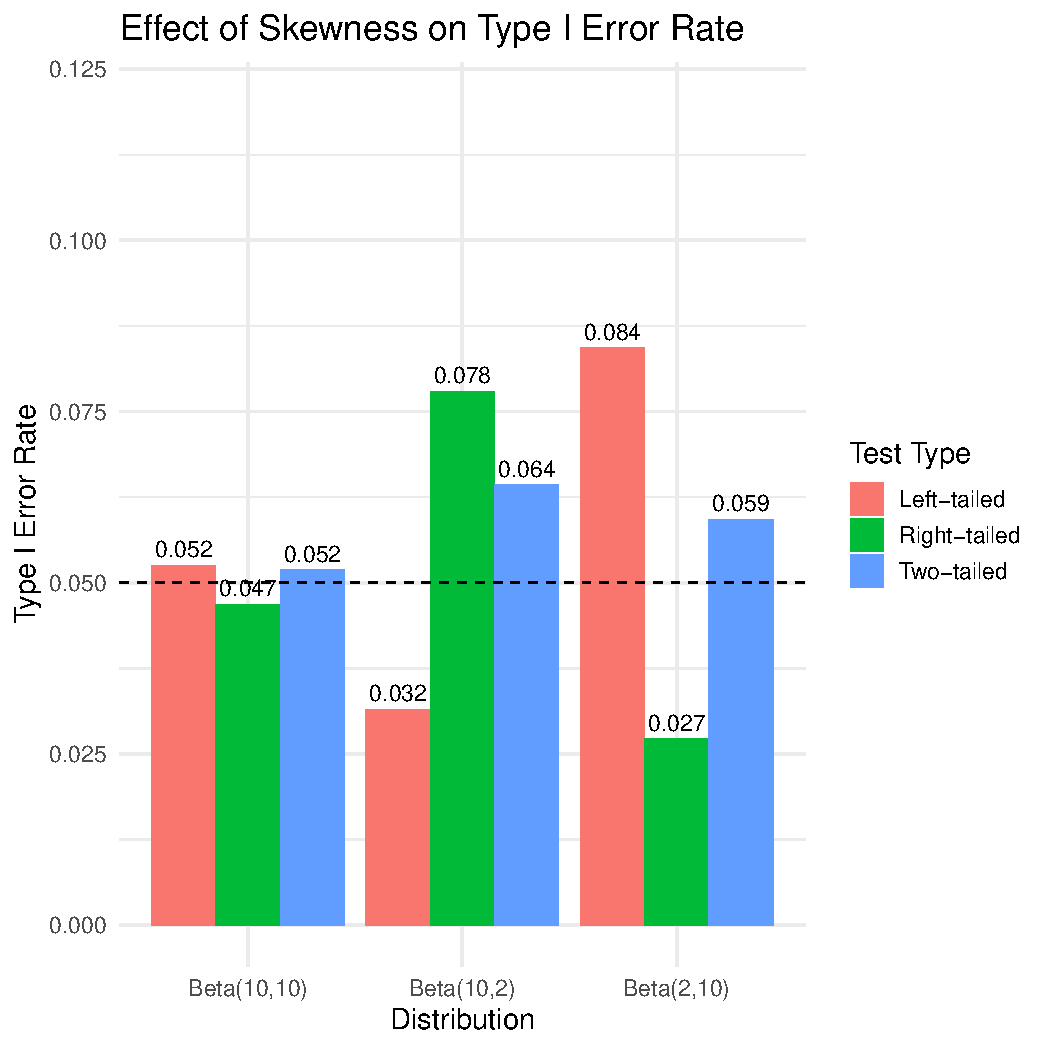
\includegraphics[width=\maxwidth]{figure/unnamed-chunk-9-1} 
\end{knitrout}
The t-test assumes that the data is symmetric, so when the data is skewed, the data becomes biased in the direction of the skew, leading to an incorrect Type 1 error.
  \end{enumerate}
%%%%%%%%%%%%%%%%%%%%%%%%%%%%%%%%%%%%%%%%%%%%%%%%%%%%%%%%%%%%%%%%%%%%%%%%%%%%%%%%
%%%%%%%%%%%%%%%%%%%%%%%%%%%%%%%%%%%%%%%%%%%%%%%%%%%%%%%%%%%%%%%%%%%%%%%%%%%%%%%%
% End Document
%%%%%%%%%%%%%%%%%%%%%%%%%%%%%%%%%%%%%%%%%%%%%%%%%%%%%%%%%%%%%%%%%%%%%%%%%%%%%%%%
%%%%%%%%%%%%%%%%%%%%%%%%%%%%%%%%%%%%%%%%%%%%%%%%%%%%%%%%%%%%%%%%%%%%%%%%%%%%%%%%
\end{enumerate}
\bibliography{bibliography}
\end{document}
